\documentclass[aspectratio=169]{beamer}

% Theme and Color Setup
\usetheme{Madrid}
\usecolortheme{whale}
\useinnertheme{rectangles}
\useoutertheme{miniframes}

% Additional Packages
\usepackage[utf8]{inputenc}
\usepackage[T1]{fontenc}
\usepackage{graphicx}
\usepackage{booktabs}
\usepackage{listings}
\usepackage{amsmath}
\usepackage{amssymb}
\usepackage{xcolor}
\usepackage{tikz}
\usepackage{pgfplots}
\pgfplotsset{compat=1.18}
\usetikzlibrary{positioning}
\usepackage{hyperref}

% Custom Colors
\definecolor{myblue}{RGB}{31, 73, 125}
\definecolor{mygray}{RGB}{100, 100, 100}
\definecolor{mygreen}{RGB}{0, 128, 0}
\definecolor{myorange}{RGB}{230, 126, 34}
\definecolor{mycodebackground}{RGB}{245, 245, 245}

% Set Theme Colors
\setbeamercolor{structure}{fg=myblue}
\setbeamercolor{frametitle}{fg=white, bg=myblue}
\setbeamercolor{title}{fg=myblue}
\setbeamercolor{section in toc}{fg=myblue}
\setbeamercolor{item projected}{fg=white, bg=myblue}
\setbeamercolor{block title}{bg=myblue!20, fg=myblue}
\setbeamercolor{block body}{bg=myblue!10}
\setbeamercolor{alerted text}{fg=myorange}

% Set Fonts
\setbeamerfont{title}{size=\Large, series=\bfseries}
\setbeamerfont{frametitle}{size=\large, series=\bfseries}
\setbeamerfont{caption}{size=\small}
\setbeamerfont{footnote}{size=\tiny}

% Code Listing Style
\lstdefinestyle{customcode}{
  backgroundcolor=\color{mycodebackground},
  basicstyle=\footnotesize\ttfamily,
  breakatwhitespace=false,
  breaklines=true,
  commentstyle=\color{mygreen}\itshape,
  keywordstyle=\color{blue}\bfseries,
  stringstyle=\color{myorange},
  numbers=left,
  numbersep=8pt,
  numberstyle=\tiny\color{mygray},
  frame=single,
  framesep=5pt,
  rulecolor=\color{mygray},
  showspaces=false,
  showstringspaces=false,
  showtabs=false,
  tabsize=2,
  captionpos=b
}
\lstset{style=customcode}

% Custom Commands
\newcommand{\hilight}[1]{\colorbox{myorange!30}{#1}}
\newcommand{\source}[1]{\vspace{0.2cm}\hfill{\tiny\textcolor{mygray}{Source: #1}}}
\newcommand{\concept}[1]{\textcolor{myblue}{\textbf{#1}}}
\newcommand{\separator}{\begin{center}\rule{0.5\linewidth}{0.5pt}\end{center}}

% Footer and Navigation Setup
\setbeamertemplate{footline}{
  \leavevmode%
  \hbox{%
  \begin{beamercolorbox}[wd=.3\paperwidth,ht=2.25ex,dp=1ex,center]{author in head/foot}%
    \usebeamerfont{author in head/foot}\insertshortauthor
  \end{beamercolorbox}%
  \begin{beamercolorbox}[wd=.5\paperwidth,ht=2.25ex,dp=1ex,center]{title in head/foot}%
    \usebeamerfont{title in head/foot}\insertshorttitle
  \end{beamercolorbox}%
  \begin{beamercolorbox}[wd=.2\paperwidth,ht=2.25ex,dp=1ex,center]{date in head/foot}%
    \usebeamerfont{date in head/foot}
    \insertframenumber{} / \inserttotalframenumber
  \end{beamercolorbox}}%
  \vskip0pt%
}

% Turn off navigation symbols
\setbeamertemplate{navigation symbols}{}

% Title Page Information
\title[Week 7: Data Processing Architectures]{Week 7: Data Processing Architectures}
\subtitle{}
\author[J. Smith]{John Smith, Ph.D.}
\institute[University Name]{
  Department of Computer Science\\
  University Name\\
  \vspace{0.3cm}
  Email: email@university.edu\\
  Website: www.university.edu
}
\date{\today}

% Document Start
\begin{document}

\frame{\titlepage}

\begin{frame}[fragile]
  \titlepage
\end{frame}

\begin{frame}[fragile]
  \frametitle{Overview of Data Processing Architectures}
  \begin{block}{Definition}
    Data processing architectures are essential frameworks that define how data is ingested, processed, and stored.
  \end{block}
  They enable organizations to efficiently handle large datasets by providing structured solutions tailored to their specific requirements.
  
  \begin{block}{Importance}
    Understanding these architectures is critical in a data-driven world where the volume of information is exponentially increasing.
  \end{block}
\end{frame}

\begin{frame}[fragile]
  \frametitle{Importance of Data Processing Architectures}
  \begin{enumerate}
    \item \textbf{Effective Handling of Large Datasets:}
    \begin{itemize}
      \item Data is generated at an unprecedented rate across various domains.
      \item Traditional techniques can falter under large volumes, necessitating robust architectures designed for scalability and performance.
    \end{itemize}
    
    \item \textbf{Optimized Resource Management:}
    \begin{itemize}
      \item Appropriate architectures ensure efficient use of computational resources, balancing workloads to avoid bottlenecks.
      \item This leads to cost savings and improved processing efficiency.
    \end{itemize}
    
    \item \textbf{Data Integrity and Consistency:}
    \begin{itemize}
      \item Different architectures maintain data integrity through mechanisms that ensure accuracy and reliability, which is crucial for real-time applications.
    \end{itemize}
    
    \item \textbf{Facilitating Real-Time Analytics:}
    \begin{itemize}
      \item Proper architectures support rapid ingestion and analysis of data, allowing timely, informed decisions.
    \end{itemize}
  \end{enumerate}
\end{frame}

\begin{frame}[fragile]
  \frametitle{Examples of Data Processing Architectures}
  \begin{itemize}
    \item \textbf{Batch Processing:}
      \begin{itemize}
        \item Data collected over time and processed in bulk.
        \item Example: An online retailer collects user purchase data for daily batch analysis to inform inventory management.
      \end{itemize}
    
    \item \textbf{Stream Processing:}
      \begin{itemize}
        \item Data processed in real-time as it comes in.
        \item Example: Stock market applications analyze trading data and execute trades automatically based on predefined criteria.
      \end{itemize}
  \end{itemize}
\end{frame}

\begin{frame}[fragile]
  \frametitle{Conclusion and Key Points}
  \begin{itemize}
    \item Data processing architectures form the backbone of data management strategies in modern organizations.
    \item Understanding differences between batch processing and stream processing is crucial for selecting the right architecture.
    \item Choosing the correct architecture impacts the efficiency, reliability, and speed of data processing tasks.
  \end{itemize}
  
  \begin{block}{Next Steps}
    Explore \textbf{Batch Processing} in detail to understand its definition, characteristics, benefits, and common use cases.
  \end{block}
\end{frame}

\begin{frame}[fragile]
    \frametitle{Batch Processing - Definition}
    \begin{block}{Definition of Batch Processing}
        Batch processing is a method of executing a series of jobs or tasks on a computer system without manual intervention, where jobs are collected and processed together (in batches). This approach is mainly used for processing large volumes of data over a specified period.
    \end{block}
\end{frame}

\begin{frame}[fragile]
    \frametitle{Batch Processing - Characteristics}
    \begin{itemize}
        \item \textbf{Non-Immediate Execution:} Jobs are accumulated and processed at once.
        \item \textbf{Scheduled Execution:} Typically runs during off-peak hours to optimize resource usage.
        \item \textbf{High Throughput:} Processes large quantities of data efficiently.
        \item \textbf{Resource Utilization:} Efficient use of system resources with multi-programming.
        \item \textbf{Minimal User Interaction:} Little to no human intervention required once submitted.
    \end{itemize}
\end{frame}

\begin{frame}[fragile]
    \frametitle{Batch Processing - Benefits and Use Cases}
    \begin{block}{Benefits of Batch Processing}
        \begin{itemize}
            \item Efficiency: Handles large volumes of data quickly with minimal overhead.
            \item Cost-Effective: Reduces operational costs by utilizing off-peak processing times.
            \item Scalability: Easily scales with increasing data volumes.
            \item Automation: Decreases potential for errors by reducing human intervention.
        \end{itemize}
    \end{block}

    \begin{block}{Use Cases of Batch Processing}
        \begin{enumerate}
            \item Payroll Processing
            \item Large Data Transformations
            \item Report Generation
            \item Data Backup
        \end{enumerate}
    \end{block}
\end{frame}

\begin{frame}[fragile]
    \frametitle{Batch Processing - Example and Key Takeaways}
    \begin{block}{Example of Batch Processing}
        In a retail environment, a batch process may run overnight to update inventory levels, generate sales reports, and apply discounts based on predetermined rules.
    \end{block}

    \begin{block}{Key Takeaways}
        \begin{itemize}
            \item Essential for managing large datasets with minimal user interaction.
            \item Suitable for applications requiring high throughput and resource optimization.
            \item Important for effective data processing architecture design.
        \end{itemize}
    \end{block}
\end{frame}

\begin{frame}[fragile]
    \frametitle{Batch Processing - Conclusion}
    Batch processing remains a fundamental approach in data processing architectures. It is especially relevant for businesses reliant on large volumes of repetitive tasks. 
    \newline 
    In the next slide, we will compare this with real-time processing to highlight the differences and appropriate use cases for each method.
\end{frame}

\begin{frame}[fragile]{Real-Time Processing - Definition}
    \begin{block}{Definition of Real-Time Processing}
        Real-time processing refers to the immediate processing of data as it is generated or received, with results available without any significant delay (typically within milliseconds to a few seconds). This approach is essential for applications that require instant feedback and decision-making based on current data.
    \end{block}
\end{frame}

\begin{frame}[fragile]{Real-Time Processing - Key Characteristics}
    \begin{block}{Key Characteristics}
        \begin{enumerate}
            \item \textbf{Immediate Response}: Data is processed instantly to allow for rapid decision-making.
            \item \textbf{Low Latency}: The system's response time is critical; latency must be minimized.
            \item \textbf{Continuous Data Flow}: Data is processed as a continuous stream rather than in batches.
            \item \textbf{High Availability}: Systems must be reliable and operational at all times since they often support critical applications.
            \item \textbf{Event-Driven}: Processes are triggered by specific events, not scheduled tasks.
        \end{enumerate}
    \end{block}
\end{frame}

\begin{frame}[fragile]{Real-Time Processing - Examples of Applications}
    \begin{block}{Examples of Applications}
        \begin{itemize}
            \item \textbf{Finance:}
                \begin{itemize}
                    \item \textit{Stock Trading}: Algorithms analyze market conditions and execute trades in real-time to capitalize on fleeting opportunities.
                \end{itemize}
                
            \item \textbf{Healthcare:}
                \begin{itemize}
                    \item \textit{Patient Monitoring Systems}: Monitor vital signs and alert medical staff to critical changes.
                \end{itemize}
                
            \item \textbf{Telecommunications:}
                \begin{itemize}
                    \item \textit{Network Monitoring}: Continuously track data traffic and detect anomalies in real-time.
                \end{itemize}
                
            \item \textbf{IoT Devices:}
                \begin{itemize}
                    \item \textit{Smart Home Systems}: Devices like smart thermostats process data instantly for adjustments or alerts.
                \end{itemize}
                
            \item \textbf{Transportation:}
                \begin{itemize}
                    \item \textit{Traffic Management}: Use real-time data to optimize traffic flow and manage traffic lights.
                \end{itemize}
        \end{itemize}
    \end{block}
\end{frame}

\begin{frame}[fragile]{Real-Time Processing - Key Points and Summary}
    \begin{block}{Key Points to Emphasize}
        \begin{itemize}
            \item Real-time processing is crucial in scenarios where timely data analysis is essential.
            \item The choice between real-time and batch processing depends on business needs and the nature of the processed data.
            \item Scalability and speed of infrastructure are vital in environments implementing real-time processing.
        \end{itemize}
    \end{block}

    \begin{block}{Summary}
        Real-time processing enables instant responses to data changes, essential for operations and decision-making in various industries.
    \end{block}
\end{frame}

\begin{frame}[fragile]
    \frametitle{Batch vs. Real-Time Processing - Overview}
    \begin{block}{Overview}
        In data processing, two primary architectures are commonly recognized: 
        \textbf{Batch Processing} and \textbf{Real-Time Processing}. 
        Understanding the distinctions between these two approaches helps organizations choose the right solution based on their specific needs.
    \end{block}
\end{frame}

\begin{frame}[fragile]
    \frametitle{Batch vs. Real-Time Processing - Key Comparisons}
    \begin{block}{Speed}
        \begin{itemize}
            \item \textbf{Batch Processing}:
                \begin{itemize}
                    \item Processes data in large volumes at once, often scheduled at specific intervals (e.g., daily, hourly).
                    \item Generally slower, as it accumulates data before processing.
                    \item \textit{Example: End-of-day report generation for financial summaries.}
                \end{itemize}
            \item \textbf{Real-Time Processing}:
                \begin{itemize}
                    \item Processes data immediately as it arrives, ensuring low latency.
                    \item \textit{Example: Online transaction processing (e.g., credit card authorizations).}
                \end{itemize}
        \end{itemize}
    \end{block}
\end{frame}

\begin{frame}[fragile]
    \frametitle{Batch vs. Real-Time Processing - Latency and Applications}
    \begin{block}{Latency}
        \begin{itemize}
            \item \textbf{Batch Processing}:
                \begin{itemize}
                    \item Higher latency; results may only be available after the batch is processed.
                    \item Suitable for applications where immediate feedback is not critical.
                \end{itemize}
            \item \textbf{Real-Time Processing}:
                \begin{itemize}
                    \item Low latency; results and insights are available almost instantaneously.
                    \item Ideal for time-sensitive applications.
                \end{itemize}
        \end{itemize}
    \end{block}
    
    \begin{block}{Suitable Applications}
        \begin{itemize}
            \item \textbf{Batch Processing}:
                \begin{itemize}
                    \item Data Warehousing
                    \item Reporting
                    \item Historical Data Analysis
                \end{itemize}
            \item \textbf{Real-Time Processing}:
                \begin{itemize}
                    \item Financial Services
                    \item Social Media Platforms
                    \item IoT Systems
                \end{itemize}
        \end{itemize}
    \end{block}
\end{frame}

\begin{frame}[fragile]
    \frametitle{Batch vs. Real-Time Processing - Summary and Takeaways}
    \begin{block}{Summary}
        \begin{tabular}{|l|l|l|}
            \hline
            Feature & Batch Processing & Real-Time Processing \\
            \hline
            Speed & Slower, processes in bulk & Fast, processes instantly \\
            \hline
            Latency & Higher, results available later & Lower, immediate insights \\
            \hline
            Suitable Applications & Reporting, Data Warehousing & Fraud Detection, IoT Monitoring \\
            \hline
        \end{tabular}
    \end{block}
    
    \begin{block}{Takeaway Points}
        \begin{itemize}
            \item Choose \textbf{Batch Processing} for applications that analyze bulk data with less urgency.
            \item Opt for \textbf{Real-Time Processing} when immediate insights are critical for decision-making.
        \end{itemize}
    \end{block}
\end{frame}

\begin{frame}[fragile]
    \frametitle{Example Illustrations}
    \begin{block}{Traffic Monitoring System}
        \begin{itemize}
            \item \textbf{Batch Processing}: Analyzes traffic data every hour to provide average speeds and congestion reports.
            \item \textbf{Real-Time Processing}: Sends alerts for accidents or unusual traffic, adjusting traffic lights dynamically.
        \end{itemize}
    \end{block}
    
    \begin{block}{Conclusion}
        In conclusion, the appropriate method of processing data—whether batch or real-time—depends on application needs, the importance of speed, and the acceptable level of latency. Understanding these differences empowers organizations to optimize their data processing strategies effectively.
    \end{block}
\end{frame}

\begin{frame}[fragile]
    \frametitle{Overview of Big Data Concepts}
    Big Data refers to the vast volumes of structured and unstructured data generated every second in the digital age. 
    The concept is defined by four key attributes: Volume, Variety, Velocity, and Value, often referred to as the "Four Vs" of Big Data.
    
    Understanding these attributes is crucial for leveraging the power of Big Data in decision-making and operations.
\end{frame}

\begin{frame}[fragile]
    \frametitle{The Four Vs of Big Data}
    \begin{enumerate}
        \item \textbf{Volume}
        \item \textbf{Variety}
        \item \textbf{Velocity}
        \item \textbf{Value}
    \end{enumerate}
    These key attributes help organizations identify and manage large datasets effectively.
\end{frame}

\begin{frame}[fragile]
    \frametitle{1. Volume}
    \begin{block}{Definition}
        Refers to the sheer amount of data created. It is not just about size but also about the ability to analyze massive datasets.
    \end{block}
    \begin{itemize}
        \item \textbf{Example}: Social media platforms produce over 500 terabytes of data per day. By 2025, it’s estimated that the world will generate 463 exabytes of data daily!
    \end{itemize}
    \textbf{Key Point}: Systems must be able to store and process this huge volume efficiently.
\end{frame}

\begin{frame}[fragile]
    \frametitle{2. Variety}
    \begin{block}{Definition}
        Indicates the different types of data generated from various sources such as text, images, video, audio, structured databases, and unstructured data.
    \end{block}
    \begin{itemize}
        \item \textbf{Example}: Data comes from social media posts, sensor data from IoT devices, transaction records, and more.
    \end{itemize}
    \textbf{Key Point}: Tools and architectures must accommodate various formats and data sources to derive meaningful insights.
\end{frame}

\begin{frame}[fragile]
    \frametitle{3. Velocity}
    \begin{block}{Definition}
        Describes the speed at which data is generated, processed, and analyzed. 
    \end{block}
    \begin{itemize}
        \item \textbf{Example}: Stock market data fluctuates every microsecond, necessitating immediate processing for accurate trading.
    \end{itemize}
    \textbf{Key Point}: Efficient data processing architectures must support both real-time and batch processing capabilities.
\end{frame}

\begin{frame}[fragile]
    \frametitle{4. Value}
    \begin{block}{Definition}
        Emphasizes the importance of extracting meaningful insights from data. 
    \end{block}
    \begin{itemize}
        \item \textbf{Example}: Companies utilizing Big Data analytics can predict consumer trends and enhance customer experiences.
    \end{itemize}
    \textbf{Key Point}: Organizations need to adopt a strategic approach to ensure they maximize the value of their data.
\end{frame}

\begin{frame}[fragile]
    \frametitle{Summary and Next Steps}
    \begin{itemize}
        \item Understanding the Four Vs of Big Data helps organizations build robust data architectures capable of storing, processing, and analyzing large and diverse datasets.
        \item This foundational understanding is crucial before delving into specific technologies that support big data processing.
    \end{itemize}
    *Next, we will explore Key Technologies in Data Processing to understand the tools and frameworks utilized in handling Big Data efficiently.*
\end{frame}

\begin{frame}[fragile]
    \frametitle{Key Technologies in Data Processing}
    \begin{block}{Overview}
        Data processing architectures are critical for handling and analyzing large volumes of data. This discussion covers two prominent technologies: 
        \textbf{Apache Hadoop} and \textbf{Apache Spark}.
    \end{block}
\end{frame}

\begin{frame}[fragile]
    \frametitle{1. Apache Hadoop}
    \begin{itemize}
        \item \textbf{Definition}: Open-source framework for storing and processing massive data sets across clusters.
        \item \textbf{Key Components}:
            \begin{itemize}
                \item \textbf{Hadoop Distributed File System (HDFS)}: 
                    \begin{itemize}
                        \item Stores data across multiple machines.
                        \item Ensures high throughput access to application data.
                    \end{itemize}
                \item \textbf{MapReduce}:
                    \begin{itemize}
                        \item A programming model for distributed processing of large data sets.
                        \item \textbf{Example}: 
                            \begin{enumerate}
                                \item \textbf{Map}: Output key-value pairs (key = word, value = 1).
                                \item \textbf{Reduce}: Sum values for each key.
                            \end{enumerate}
                    \end{itemize}
                \end{itemize}
        \item \textbf{Strengths}:
            \begin{itemize}
                \item \textbf{Scalability}: Handles petabytes of data by adding more nodes.
                \item \textbf{Fault Tolerance}: Data is automatically replicated across nodes.
            \end{itemize}
    \end{itemize}
\end{frame}

\begin{frame}[fragile]
    \frametitle{2. Apache Spark}
    \begin{itemize}
        \item \textbf{Definition}: Open-source distributed computing system optimized for in-memory processing.
        \item \textbf{Key Features}:
            \begin{itemize}
                \item \textbf{In-Memory Computation}: Processes data faster than Hadoop by caching.
                \item \textbf{Unified Engine}: Supports batch processing, real-time streaming, machine learning, and graph processing.
            \end{itemize}
        \item \textbf{Programming Models}:
            \begin{itemize}
                \item \textbf{Resilient Distributed Datasets (RDDs)}: Core abstraction for distributed processing.
                \item \textbf{Transformations and Actions}:
                    \begin{itemize}
                        \item \textbf{Transformations}: Create new RDD (e.g., \texttt{map, filter}).
                        \item \textbf{Actions}: Trigger computation (e.g., \texttt{count, collect}).
                    \end{itemize}
            \end{itemize}
    \end{itemize}
\end{frame}

\begin{frame}[fragile]
    \frametitle{Example: Word Count with Spark}
    \begin{block}{Simplified Code Example}
    \begin{lstlisting}[language=Python]
from pyspark import SparkContext

sc = SparkContext("local", "WordCount")
text_file = sc.textFile("path/to/textfile.txt")
counts = text_file.flatMap(lambda line: line.split()) \
                  .map(lambda word: (word, 1)) \
                  .reduceByKey(lambda a, b: a + b)
counts.saveAsTextFile("output/path")
    \end{lstlisting}
    \end{block}
\end{frame}

\begin{frame}[fragile]
    \frametitle{Key Points to Emphasize}
    \begin{itemize}
        \item \textbf{Purpose}: Both Hadoop and Spark are essential for big data processing but serve different needs.
        \item \textbf{Speed vs. Scalability}: 
            \begin{itemize}
                \item Hadoop excels in storage and fault tolerance.
                \item Spark is faster due to in-memory processing.
            \end{itemize}
        \item \textbf{Flexibility}: Spark handles various data processing tasks beyond batch jobs.
    \end{itemize}
\end{frame}

\begin{frame}[fragile]
    \frametitle{Conclusion}
    Understanding the strengths and functionalities of Hadoop and Spark is essential for designing effective data processing architectures. With the growth of big data, these technologies enable organizations to fully leverage their data.
\end{frame}

\begin{frame}[fragile]
    \frametitle{Architectural Considerations for Data Processing}
    \begin{block}{Best Practices for Designing Scalable and Efficient Data Processing Architectures}
        \begin{enumerate}
            \item Modular Design
            \item Scalability
            \item Data Storage Considerations
            \item Data Processing Frameworks
            \item High Availability and Fault Tolerance
            \item Efficient Data Flow Management
            \item Data Governance and Security
            \item Monitoring and Performance Tuning
        \end{enumerate}
    \end{block}
\end{frame}

\begin{frame}[fragile]
    \frametitle{1. Modular Design}
    \begin{itemize}
        \item \textbf{Explanation}: 
            Break the data processing architecture into smaller, independent modules or components. Each module can be developed, tested, and scaled independently.
        \item \textbf{Example}: 
            In a data pipeline, separate extraction, transformation, and loading (ETL) processes. This allows for easier updates and maintenance.
    \end{itemize}
\end{frame}

\begin{frame}[fragile]
    \frametitle{2. Scalability}
    \begin{itemize}
        \item \textbf{Explanation}: 
            Ensure that the architecture can scale effectively in response to increasing data volumes or user requests.
        \item \textbf{Key Considerations}:
            \begin{itemize}
                \item Vertical Scaling: Upgrade existing hardware (more CPU, memory).
                \item Horizontal Scaling: Add more machines to distribute load.
            \end{itemize}
        \item \textbf{Example}: 
            Using cloud services like AWS or Azure allows for automatic scaling based on demand.
    \end{itemize}
\end{frame}

\begin{frame}[fragile]
    \frametitle{3. Data Storage Considerations}
    \begin{itemize}
        \item \textbf{Explanation}: 
            Choose the right storage method based on access frequency and type of data.
        \item \textbf{Options}:
            \begin{itemize}
                \item Data Lakes: For large volumes of raw data, such as logs (unstructured).
                \item Data Warehouses: For optimized, structured data for analysis and reporting.
            \end{itemize}
        \item \textbf{Example}: 
            Use Amazon S3 for data lakes and Amazon Redshift for data warehousing.
    \end{itemize}
\end{frame}

\begin{frame}[fragile]
    \frametitle{4. Data Processing Frameworks}
    \begin{itemize}
        \item \textbf{Explanation}: 
            Utilize efficient data processing frameworks that are well-suited for your use case.
        \item \textbf{Examples}:
            \begin{itemize}
                \item Apache Hadoop: Best for batch processing of large datasets.
                \item Apache Spark: Ideal for real-time data processing and analytics.
            \end{itemize}
        \item \textbf{Key Point}: 
            Understand the strengths and weaknesses of each framework to pick the right one.
    \end{itemize}
\end{frame}

\begin{frame}[fragile]
    \frametitle{5. High Availability and Fault Tolerance}
    \begin{itemize}
        \item \textbf{Explanation}: 
            Design the architecture to withstand hardware failures and ensure continuous data processing.
        \item \textbf{Implementation}:
            \begin{itemize}
                \item Redundant systems to take over when one fails.
                \item Data replication across nodes.
            \end{itemize}
        \item \textbf{Example}: 
            Use clusters with failover mechanisms to keep services running in case of failures.
    \end{itemize}
\end{frame}

\begin{frame}[fragile]
    \frametitle{Summary and Conclusion}
    \begin{block}{Summary}
        Designing efficient and scalable data processing architectures requires careful consideration of modular design, scalable infrastructures, proper storage selection, reliable processing frameworks, fault tolerance, efficient data flow management, governance, and continuous performance tuning. By adhering to these best practices, organizations can ensure that their data architectures remain robust and responsive to changing demands.
    \end{block}
\end{frame}

\begin{frame}[fragile]
    \frametitle{Case Studies - Introduction}
    \begin{block}{Introduction to Data Processing Architectures}
        Data processing architectures are frameworks enabling efficient collection, processing, storage, and analysis of large data volumes. Successful implementations enhance decision-making, operational efficiency, and customer satisfaction.
    \end{block}
\end{frame}

\begin{frame}[fragile]
    \frametitle{Case Study 1: Netflix}
    \begin{block}{Overview}
        \begin{itemize}
            \item \textbf{Challenge}: Handling massive amounts of data for personalized content recommendations.
            \item \textbf{Architecture}: Hybrid cloud-based architecture using AWS.
            \item \textbf{Implementation}:
            \begin{itemize}
                \item Utilizes microservices for user preferences, streaming, and content delivery.
                \item Real-time and batch data processing using Apache Kafka and Amazon S3.
            \end{itemize}
        \end{itemize}
    \end{block}
    \begin{block}{Outcomes}
        \begin{itemize}
            \item Enhanced user engagement with tailored recommendations.
            \item Scalability to support global viewers during peak times (e.g., new releases).
        \end{itemize}
    \end{block}
    \begin{block}{Key Point}
        Netflix exemplifies the effectiveness of a microservices architecture combined with cloud scalability in delivering seamless user experiences.
    \end{block}
\end{frame}

\begin{frame}[fragile]
    \frametitle{Case Study 2: Uber}
    \begin{block}{Overview}
        \begin{itemize}
            \item \textbf{Challenge}: Managing dynamic pricing and routing while processing user and vehicle data.
            \item \textbf{Architecture}: Event-driven architecture using Apache Kafka.
            \item \textbf{Implementation}:
            \begin{itemize}
                \item Real-time data streaming processes millions of ride requests.
                \item Machine learning models predict demand and optimize pricing.
            \end{itemize}
        \end{itemize}
    \end{block}
    \begin{block}{Outcomes}
        \begin{itemize}
            \item Improved efficiency in ride matching.
            \item Real-time analytics enhance customer satisfaction with reduced wait times.
        \end{itemize}
    \end{block}
    \begin{block}{Key Point}
        Uber's event-driven architecture allows for real-time data processing and agile adaptations to changing conditions.
    \end{block}
\end{frame}

\begin{frame}[fragile]
    \frametitle{Case Study 3: Airbnb}
    \begin{block}{Overview}
        \begin{itemize}
            \item \textbf{Challenge}: Analyzing user interactions for better service offerings.
            \item \textbf{Architecture}: Data lake architecture based on Hadoop.
            \item \textbf{Implementation}:
            \begin{itemize}
                \item Centralized storage accumulates data from various sources.
                \item Bidirectional data flow supports real-time updates and historical queries.
            \end{itemize}
        \end{itemize}
    \end{block}
    \begin{block}{Outcomes}
        \begin{itemize}
            \item Improved marketing strategies through insights into user behavior.
            \item Enhanced data-driven decision-making for better rental matching.
        \end{itemize}
    \end{block}
    \begin{block}{Key Point}
        Airbnb's data lake architecture supports comprehensive analysis and transforms raw data into actionable insights.
    \end{block}
\end{frame}

\begin{frame}[fragile]
    \frametitle{Conclusion and Key Takeaways}
    \begin{block}{Conclusion}
        Organizations adopting effective data processing architectures show significant improvements in operations and user experiences. The case studies of Netflix, Uber, and Airbnb illustrate how tailored architectures meet diverse data processing needs.
    \end{block}
    \begin{block}{Key Takeaways}
        \begin{itemize}
            \item \textbf{Flexibility and Scalability}: Choose architectures that can scale with user demand.
            \item \textbf{Real-Time Processing}: Leverage streaming technologies for immediate insights.
            \item \textbf{Data-Driven Decisions}: Ensure data architectures support robust analytics capabilities.
        \end{itemize}
    \end{block}
\end{frame}

\begin{frame}[fragile]{Introduction to Future Trends in Data Processing}
    \begin{block}{Overview}
        As the landscape of data processing evolves, two significant trends are:
        \begin{itemize}
            \item \textbf{Serverless Architectures}
            \item \textbf{Data Mesh}
        \end{itemize}
        Understanding these trends is crucial for anyone involved in data science and architecture.
    \end{block}
\end{frame}

\begin{frame}[fragile]{Serverless Architectures}
    \begin{block}{Definition}
        Serverless architecture is a cloud computing model where developers build and run applications without managing servers.
    \end{block}
    
    \begin{block}{Key Features}
        \begin{itemize}
            \item \textbf{Automatic Scaling:} Scales up or down based on demand.
            \item \textbf{Cost-Efficiency:} Pay only for the compute time consumed.
            \item \textbf{Focus on Code:} Developers can concentrate on writing code without server management concerns.
        \end{itemize}
    \end{block}
    
    \begin{block}{Example}
        AWS Lambda is a serverless computing service that runs code in response to events such as API calls.
    \end{block}
    
    \begin{block}{Illustration}
        \begin{center}
        User Interaction $\rightarrow$ AWS Lambda (function triggered) $\rightarrow$ Data Processing $\rightarrow$ Result (response back to user)
        \end{center}
    \end{block}
\end{frame}

\begin{frame}[fragile]{Data Mesh}
    \begin{block}{Definition}
        Data mesh is a decentralized approach to data architecture emphasizing domain-oriented ownership.
    \end{block}
    
    \begin{block}{Key Features}
        \begin{itemize}
            \item \textbf{Decentralization:} Each team owns its own data domain.
            \item \textbf{Interoperability:} Promotes creation of interoperable data products across teams.
            \item \textbf{Scalability:} Reduces bottlenecks typical in centralized architectures.
        \end{itemize}
    \end{block}
    
    \begin{block}{Example}
        Separate teams for marketing and sales manage their respective data with a focus on creating data products.
    \end{block}
    
    \begin{block}{Illustration}
        \begin{center}
            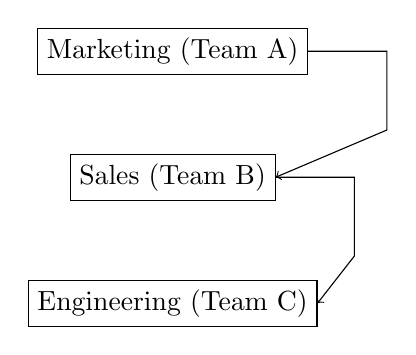
\begin{tikzpicture}
                \node (teamA) [draw] {Marketing (Team A)};
                \node (teamB) [draw, below=of teamA] {Sales (Team B)};
                \node (teamC) [draw, below=of teamB] {Engineering (Team C)};
                \draw[->] (teamA.east) -- ++(1,0) -- ++(0,-1) -- (teamB.east);
                \draw[->] (teamB.east) -- ++(1,0) -- ++(0,-1) -- (teamC.east);
            \end{tikzpicture}
        \end{center}
        Data Products (APIs)
    \end{block}
\end{frame}

\begin{frame}[fragile]{Key Points to Emphasize}
    \begin{itemize}
        \item \textbf{Serverless architectures} enhance agility and reduce costs.
        \item \textbf{Data mesh} promotes a collaborative approach to data management using domain expertise.
        \item Both trends represent significant shifts towards scalable, efficient, and collaborative architectures.
    \end{itemize}
\end{frame}

\begin{frame}[fragile]{Wrap-Up}
    Embracing serverless models and data mesh principles can significantly enhance data processing capabilities, 
    providing organizations with a competitive advantage in a data-centric world.
\end{frame}

\begin{frame}[fragile]{Conclusion - Summary of Key Points}
  \begin{block}{Understanding Data Processing Architectures}
    Data processing architectures are frameworks that define how data is collected, processed, and analyzed. These architectures are crucial for data science, influencing data accessibility, performance efficiencies, and scalability.
  \end{block}
\end{frame}

\begin{frame}[fragile]{Conclusion - Types of Data Processing Architectures}
  \begin{block}{1. Batch Processing}
    Involves processing large volumes of data collected over time in scheduled intervals. \\
    \textbf{Example:} Monthly sales data analysis where reports are generated at the end of each month.
  \end{block}

  \begin{block}{2. Stream Processing}
    This architecture processes data in real-time, allowing for immediate insights. \\
    \textbf{Example:} Stock market analysis where trades must be evaluated as they happen.
  \end{block}

  \begin{block}{3. Lambda Architecture}
    Combines batch and stream processing to provide a comprehensive view of data by processing both real-time and historical data. \\
    \textbf{Example:} A recommendation system that continuously updates based on user behavior while leveraging historical data for accuracy.
  \end{block}
\end{frame}

\begin{frame}[fragile]{Conclusion - Impact of Emerging Trends and Relevance}
  \begin{block}{Impact of Emerging Trends}
    \begin{itemize}
      \item \textbf{Serverless Architectures:} Enable developers to build applications without managing server infrastructure, thereby focusing more on data processing logic.
      \item \textbf{Data Mesh Concepts:} Promote decentralized data ownership and architecture, improving accessibility across teams.
    \end{itemize}
  \end{block}

  \begin{block}{Relevance to Data Science}
    Efficient data processing architectures are fundamental in data science for:
    \begin{itemize}
      \item Enabling rapid data analysis
      \item Driving informed decision-making
      \item Improving predictive modeling
    \end{itemize}
  \end{block}
\end{frame}

\begin{frame}[fragile]{Conclusion - Key Takeaways and Formula}
  \begin{block}{Key Takeaways}
    \begin{itemize}
      \item Choose the right data processing architecture based on your project requirements.
      \item Stay informed about emerging trends to leverage the best practices in data processing.
      \item Understand the balance between performance, scalability, and cost in production scenarios.
    \end{itemize}
  \end{block}

  \begin{block}{Formula: Rate of Data Processing}
    The metric for evaluating efficiency of data processing architectures:
    \begin{equation}
      \text{Throughput} = \frac{\text{Total Data Processed (in bytes)}}{\text{Time Taken (in seconds)}}
    \end{equation}
  \end{block}
\end{frame}


\end{document}